% !TEX program = xelatex
\documentclass[11pt,a4paper,notitlepage]{report}
\usepackage{polyglossia}
\usepackage{fontspec}
\usepackage{subfig}
\usepackage{url}
\usepackage{hyperref}
\usepackage[round]{natbib}
\usepackage[nottoc,notlot,notlof]{tocbibind}

% natbib link joining; somewhat breaks \cite, \citet
\makeatletter
\renewcommand\hyper@natlinkbreak[2]{#1}
\makeatother

\usepackage{geometry}
\geometry{%
	includeheadfoot,
	margin=1in
}

\def\TODO{{\bf ??? }}

\title{Systems and Approaches for Question Answering}
\author{Mgr. Petr Baudiš}

\begin{document}
\maketitle

\begin{abstract}%
	I define and explore the task of Factoid Question Answering.
	This involves understanding a naturally phrased question
	about some (often open domain) fact, looking this fact up
	in a knowledge base (structured database or unstructured
	text corpus), and scoring the candidate answers.
	I survey the recent scientific work and directions in this
	field, define some interesting sub-tasks and propose a new dataset.
	I then present my own baseline QA pipeline YodaQA that
	combines both structured and unstructured approaches.
	Based on experiences with this baseline and survey of the
	field, I propose some scientifically promising lines of further
	QA research.
\end{abstract}

% errata:
% - missing answer F1 for YodaQA on WebQuestions
% - in survey, missing descriptions of more unstructured and other systems,
%   and entity linking survey; in general, the survey should be considered preliminary, developed in https://github.com/brmson/qasurvey
% - YodaQA description not completely up-to-date! label-lookup, decforests with entity classification

\tableofcontents

\chapter{Introduction}
\label{ch:intro}

TODO some nice quote

In this report, I would like to propose a doctoral thesis to write
and defend at the Czech Technical University on the topic of question
answering systems.

This thesis proposal is a little unusual since I have radically changed
the topic of my research in the course of my second year of study:
from portfolio-based function optimization to question answering systems.
Therefore, the bulk of my research results published up to now are not
on topic of the proposed thesis.  I shall at least briefly showcase
the main points of my past research in the next section,
after which I exclusively focus at the topic of question answering
and propose a thesis on this topic.

\section{Portfolio-Based Optimization}

The initial focus of my doctoral research
was developing algorithm portfolio strategies
with applications particularly in continuous black-box optimization.
The results of my work have been a software framework for experiments
\cite{COCOpf}
and two results published at top-tier conferences \cite{optpf,ndsqistep}.
This research had been primarily supervised by Dr. Petr Pošík.

Let us consider the problem of finding a minimum value of a continuous
real-parameter function that has inaccessible analytical form.%
\footnote{No analytical form implies that we do not have information
e.g.\ on the derivatives of the function, except approximating
them numerically.}
This is a rich area of research that produced many algorithms over
the last 50 years --- from the venerable Nelder-Mead simplex
algorithm \cite{NM1} to various gradient descent methods to
population-based methods.

\subsection{Online Black-box Algorithm Portfolios}

The key question in the face of such variety of optimization
algorithms is ``which algorithm should I choose?''
Unified comparison benchmarks \cite{COCO1}
can help determining the best option for a particular function class.
However, if a function is truly ``black-box'' and its features
are hard to predict, an automated process with minimum overhead
is certainly desirable.

The problem of algorithm selection is not new \cite{Rice}
and was so far popular mainly when applied to
combinatorial problem solvers \cite{combpfsurvey}.
In my work, I adopted the prism of algorithm portfolios \cite{algportfolios}
with \textit{online} selection.%
\footnote{The concept of offline selection also occurs in the literature,
	when we assume a stream of function instances and apply just a single
	algorithm on each of the instances.}
That is, multiple diverse optimization algorithms are applied
to the given function instance simultaneously, with the best
performers quickly gaining the largest time allocation (that is,
the chance to perform the most optimization steps).

Deciding which algorithm to apply in each step of the portfolio
optimization is essentialy an instance of the well-known Multi-Armed
Bandit Problem, where a policy decides which algorithm to try next
based on their empirically determined expected reward.
I have built a modular Python framework \textbf{COCOpf} \cite{COCOpf}
suitable both for research and application of this problem.

This helped me to identify fine structure of the problem
(particularly, I proposed a classification of functions based on
their in-portfolio behavior).
Further, I have built a reference portfolio of seven well-known
diverse optimization algorithms and based on performance evaluation
using the popular COCO optimization benchmark \cite{COCO1}, I have
identified a policy that significantly improves the baseline and
on well-behaved functions on average overperforms even the overally
best individual algorithm. This result was presented at the
PPSN 2014 conference. \cite{optpf}

\subsection{Minimizing Separable Functions by a Mix of Methods}

Another tier of research on how to best combine different optimization
algorithms concerns speeding up optimization of continuous black-box
\textit{separable} functions in particular.  I have closely cooperated
on this research with my supervisor, Dr. Petr Pošík.

Separable multivariate functions can be decomposed to a sum of univariate
functions, each parametrized solely by a single dimension of the input
vector.
For some very hard separable functions, exploiting separability
is the only way to quickly find the minimum and a natural idea to optimize
such functions is to use univariate optimization algorithms on individual
dimensions.
In \cite{PosikGECCO2009LineSearch}, Brent's method \cite{Brent1973} and the STEP algorithm \cite{STEP} were used to separately optimize the function along each dimension.
Brent's method was shown to be fast in case of unimodal functions, but due to its local nature it fails on multimodal functions.
The global STEP method was able to solve both the uni- and multimodal functions, but needed much larger number of function evaluations.
Moreover, their multidimensional variants were constructed inefficiently: the dimensions were optimized sequentially, one by one.

We have built on the above mentioned methods, and contributed two improvements:

\begin{enumerate}
	\item We combined Brent's method and STEP into a single algorithm which converges faster than STEP (in many cases, it is almost as fast as Brent's method), while it preserves the global search ability of STEP (thus solving a larger proportion of functions than Brent's method, and often doing it faster).

	\item We suggested a better way of making a multidimensional variant of this method. As opposed to solving the 1D problem in all dimensions sequentially, we proposed to interleave the steps in individual dimensions, updating the full coordinates of sampled points based on results obtained in other dimensions so far.
\end{enumerate}

Thus, we have introduced a new hybrid algorithm ``Brent-STEP'' combining
these two methods non-trivially and demonstrated that
on univariate and separable functions the hybrid algorithm
in general outperforms both of them,
in the univariate case often by a wide margin,
and that it is behaving robustly even when one of the constituent methods
is failing to converge.
This result was presented at the GECCO 2015 conference.
\cite{ndsqistep}

\section{Question Answering}

The current focus of my doctoral research
is improving the state-of-art in the field of factoid question answering.
My main results so far have been
building an extensive question answering system \textbf{YodaQA} \cite{YodaQAPoster2015}
and proposing a high-quality dataset \cite{YodaQACLEF2015},
but I have also applied the system to a biological QA domain \cite{YodaQABioASQ2015}
and achieved some new results not published yet (described later in the proposal).
This research is primarily supervised by Dr. Jan Šedivý;
some of the newest results have been achieved while collaborating
with intern students in our group.

\subsection{Factoid Question Answering}

Let us consider the Question Answering problem --- a function of
unstructured user query that returns the information queried for.
This is a harder problem than a linked data graph search (which requires
a precisely structured user query) or a generic search engine (which
returns whole documents or sets of passages instead of the specific
information).

The Question Answering task is however a natural extension of a search
engine, as currently employed e.g.\ in Google Search \cite{googleKG}
or personal assistants like Apple Siri, and with the high
profile IBM Watson Jeopardy! matches \cite{WatsonOverview}
it has became a benchmark of progress in AI research.

My goal is ultimately building a general purpose QA system.
Thus, I consider an ``open domain'' general factoid question answering,
rather than domain-specific applications, though keeping flexibility
in this direction is certainly worthwhile.

TODO some examples of questions and answers

\subsection{Task Outline}

Diverse QA system architectures have been proposed in the last 15 years,
applying different approaches to information retrieval.  A full survey
follows, for now let me outline at least the most basic choices I faced
when designing my system.

First, the restriction to \textbf{factoid} questions means the system
is essentially an extension of a search engine (rather than deducing
facts logically) and should return precisely specified, relatively short
text snippets as short answers.  Answering happens mainly based on fact
lookup.  This is in contrast with different question answering tasks
(like Language Comprehension Entrance Exams) where the system needs to
process a text passage and answer tricky questions about the text meaning
(see Sec.~\ref{sec:nonfactoid}).

Perhaps the most popular approach in factoid QA research has been restricting
the task to querying structured knowledge bases, typically using the
RDF paradigm and accessible via SPARQL\@.  The QA problem can
be then rephrased as learning a function translating free-text user query
to a structured lambda expression or SPARQL query. \cite{Semantic2013Berant, Semantic2014Bordes}
I prefer to focus on unstructured datasets as the coverage of the system
as well as domain versatility increases dramatically; building a combined
portfolio of structured and unstructured knowledge bases
is then again an obvious extension.

When relying on unstructured knowledge bases, a common strategy is to offload
the information retrieval on an external high-quality web search engine
like Google or Bing (see e.g.\ the \textbf{AskMSR} system \cite{AskMSR}
or many others).
I make a point of relying purely on local information sources.%
\footnote{However, as non-benchmarked extension, YodaQA also includes
	Bing search as described in Sec.~\ref{sec:bing}.}
While the task becomes noticeably harder,
I believe the outcome is a more
universal system that could be readily refocused on a specific domain
or proprietary knowledge base, and also a system more appropriate as
a scientific platform as the results are fully reproducible over time.

Finally, a common restriction of the QA problem concerns only selecting
the most relevant answer-bearing passage, given a tuple of input question
and set of pre-selected candidate passages \cite{WangQAGrammar}.
This Answer Sentence Selection task is certainly
worthwhile as a component of a QA system but does not form a full-fledged
system by itself.
It may be argued that returning a whole passage is more useful for the user than a direct narrow answer,
but this precludes any reasoning or other indirect answer synthesis on the part of the system,
while the context and supporting evidence can be still provided by the user interface.
Direct answer output may be also used in a more general AI reasoning engine,
an idea that I keep in sight within my design though it is clearly
out of scope for the thesis I propose.

To summarize, the system I propose should produce short, clear answers
based on information retrieval from both
unstructured (full-text) and structured (database) knowledge bases,
and not rely on any ``omniscient web search'' to make the task easier
specifically in the open domain setting.

\section{This Thesis Proposal}

The rest of this proposal shall focus on building the case for
a thesis on the topic of factoid question answering.
Chapter~\ref{ch:survey}
surveys the field in detail, examining different formulations of the problem
as well as a variety of sub-tasks, reference datasets and approaches,
and recent progress in the field.
Chapter~\ref{ch:work} describes
the work I have done on the thesis so far --- this revolves mainly around
the question answering system YodaQA that I have built, but also progress
on some of the QA sub-tasks.
Chapter~\ref{ch:plan} outlines some of the specific problems of QA
to focus on in the thesis.
I conclude the proposal with a summary in Chapter~\ref{ch:concl}.

\chapter{State of the Art in Factoid Question Answering}
\label{ch:survey}

Basic division:  Querying for answers on structured knowledge bases,
finding answers in unstructured (text) data.

TODO more existing systems

The classic QA system \textbf{OpenEphyra} \cite{Ephyra2006}
operates on the basis of fixed question categories with hand-crafted rules,
and puts emphasis on querying web search engines.
The \textbf{OAQA} initiative \cite{OAQATowards} has developed a basic QA framework,
but does not provide an end-to-end pipeline and its usage of UIMA has
in our opinion severe design limitations (see below).
The \textbf{WatsonSim} system \cite{WatsonSim} has begun developing independently
during the course of our own work and it works on Jeopardy! statements rather
than questions.

\textbf{Jacana} \cite{TreeEdit2013Yao} \cite{TreeEditIR2013Yao}
is a promising set of loosely coupled QA-related methods
and algorithms, focused on machine learning of textual entailment.  It is
not meant to be a full QA framework and using it as an end-to-end pipeline
is not straightforward, but integration of the Jacana implementation as
modules in YodaQA is our long-term plan.

\textbf{OpenQA} \cite{OpenQA} is a recently introduced end-to-end QA pipeline platform
also developed independently during the course of our work, and shares our
goal of a common research platform in the field.  However, the approach
is very different, as OpenQA is more of a portfolio-style engine with
mostly independent pipelines which have their candidate answers combined,
while YodaQA emphasizes modularity on the pipeline stage level,
with e.g.\ all answer producers sharing a common answer analysis stage.



\section{Structured Data QA}

Benchmark:  WebQuestions (pre-determined splits), TREC (various years, curated version, \dots), WikiAnswers.

Measure: Precision, p@1, recall, F1

Bordes et al. \cite{Semantic2014Bordes} sums up:
\textit{%
The state-of-the-art techniques in open QA can be classified into two main
classes, namely, information retrieval based and semantic parsing based. Information
retrieval systems first retrieve a broad set of candidate answers by querying
the search API of KBs with a transformation of the question into a valid
query and then use fine-grained detection heuristics to identify the exact answer
(Kolomiyets survey 2011, Unger et al. 2012 templates, \cite{TreeFreebase2014Yao}).
On the other hand, semantic parsing methods focus on the correct
interpretation of the meaning of a question by a semantic parsing system. A
correct interpretation converts a question into the exact database query that
returns the correct answer. Interestingly, recent works \cite{Semantic2013Berant} \cite{SPBerant2014Paraphrase} \cite{OQA} have shown that
such systems can be efficiently trained under indirect and imperfect supervision
and hence scale to large-scale regimes, while bypassing most of the annotation
costs.}

These two approaches (IE vs. SP) have been further compared in \cite{FreebaseQA2014Yao}
and seem roughly comparable.

\subsection{IE For Structued Data}

\textbf{Information Extraction over Structured Data: Question Answering with Freebase (Jacana Freebase)} \cite{TreeFreebase2014Yao}
	--- TODO.
		Open source.

\textbf{Lean Question Answering over Freebase from Scratch (kitt.ai)} \cite{LeanFreebaseYao}
	--- simple fuzzy string matching to identify Freebase concepts,
		bag-of-words logistic regression to identify relations.
		WebQuestions F1 Berant 44.3\%, F1 Yao 53.5\%.

\subsection{SP For Structured Data}

\textbf{Open Question Answering Over Curated and Extracted Knowledge Bases (OQA)} \cite{OQA}
	--- paraphrase (mined operators) $\to$ parse (templates) $\to$ rewrite (mined operators) $\to$ execute (ensemble of KBs).
	Novel machine learning for inference and answer scoring with hidden variables.
	Datasets public, open source.
	WebQuestions F1 35\%, TREC F1 29\%, WikiAnswers F1 8\%.

\textbf{(Paralex)} \cite{Fader2013Paraphrase}

\textbf{(SEMPRE)} \cite{SPBerant2014Paraphrase}

\section{Unstructured Data QA}

When dealing with question answering on top of unstructured data,
two research directions exist: aside of generating a crisp answer,
\textit{Answer Sentence Selection} is a popular sub-task%
\footnote{\url{http://aclweb.org/aclwiki/index.php?title=Question_Answering_\%28State_of_the_art\%29}}
where instead of the answer, just an appropriate answer-bearing passage
is to be returned to the user.

\subsection{Answer Sentence Selection}

Binary classification or ranking problem.
TODO TREC-based dataset by Wang et al.
MAP and MRR reported.

\textbf{(Jacana)} \cite{TreeEdit2013Yao}

\textbf{Deep Learning for Answer Sentence Selection} \cite{Yu2014Deep}
	--- given vector embeddings $\mathbf{q}, \mathbf{a}$, estimate
	$P(rel|q,a) = \sigma(\mathbf{q}^T \mathbf{M}\, \mathbf{a} + b)$
	i.e.\ train a model with parameters $\mathbf{M}, b$ that
	generates a likely question embedding using $\mathbf{M}\, \mathbf{a}$
	and then using dot-product measures its distance to the posed question.
	Cross entropy over all QA pairs is used as the loss function for training.
	Off-the-shelf $d=50$ distributed representations by Collobert and Weston 2008
	are used as word embeddings.
	To generate compositional embeddings,
	a simple unigram model that averages the embeddings is the baseline;
	as a small ($\Delta 0.02$) improvement, bigram model is proposed that uses a CNN
	on the sentence with a bigram convolutional layer and an average-pooling layer.
	To deal with numbers and proper nouns, a token co-occurrence counter
	feature is also used; the learnt method gives $\Delta 0.125$ against this baseline.
	TREC MAP 0.7113, MRR 0.7846.

\subsection{Precise Answer Production}

TREC benchmark.  Curated TREC.  WebQuestions also possible(?).

\textbf{(DeepQA IBM Watson)} \cite{WatsonOverview}

\textbf{(Jacana)} \cite{TreeEdit2013Yao} \cite{TreeEditIR2013Yao}

\textbf{Web-based Question Answering: Revisiting AskMSR (AskMSR+)}

\textbf{Open Domain Question Answering via Semantic Enrichment (QuASE)} \cite{QuASE}
	--- web-based QA system that links snippet pieces to Freebase entities
	\textit{(entity linking)} to generate extra features for answers.
	One feature is the cosine similarity of word
	vectors corresponding to question (and web-fetched question support)
	and answer's textual propreties (like \textit{description}) in Freebase
	(N.B. word frequency vectors, not embeddings!).
	Another feature is probabilistic type matching by bag of words Bayes model
	with Perplexity.  Generative mixture model with Dirichlet priors is used
	for answer scoring.  Compared to naive web search baseline, TREC F1
	improvement was 3.5\%.  (Absolute numbers not comparable due to
	sub-sampling and re-evaluation.)

\textbf{YodaQA: A Modular Question Answering System Pipeline} \cite{YodaQAPoster2015}

\textbf{MemNets} though I still think it's a toy task in QA context.

\section{Auxiliary Tasks in QA}

\subsection{Question Classification}

In datasets which ask mostly uniform types of answers (e.g. WebQuestions,
where the answer is always an entity), it may be possible to use the same
set of features to produce and score answers across all questions.
However, e.g.\ in the TREC dataset, types of answers vary widely and
different strategies might be appropriate (even if they are to be machine
learned rather than hardcoded, as was common in the early systems).

One approach is to classify an answer to a fixed set of categories.
A two-level (coarse, fine) taxonomy based on the TREC set of questions and a labelled dataset%
\footnote{\url{http://cogcomp.cs.illinois.edu/Data/QA/QC/}}
was introduced by \textbf{Learning question classifiers} \cite{QCLearning}.
They set a baseline of coarse $P_1=91.0\%$, fine $P_1=84.2\%$.

This sentence classification problem has been one of the standard benchmarks
for semantic NLP tasks:
\begin{itemize}
	\item SVM$_S$ (Silva et al., 2011) TODO coarse $P_1=95.0\%$
	\item DCNN \cite{QtcDCNN} TODO coarse $P_1=93.0\%$
	\item CNN \cite{CNNSentClass} coarse $P_1=93.6\%$
	\item Skip-Thought Vectors \cite{SkipThought} coarse $P_1=92.2\%$ (but unsupervised)
	\item Self-Adaptive Hierarchical Sentence Model \cite{AdaSent} (AdaSent) coarse $P_1=92.6\%$
	\item TODO more papers; \cite{AdaSent} has some references; separate embedding and classical?, supervised and unsupervised; even primitive baseline is something like $85\%$
\end{itemize}

A different approach that was introduced by IBM Watson DeepQA \cite{WatsonTyCor}
associates the question with a Lexical Answer Type (LAT) which is
an arbitrary English word that would describe the answer concept
(e.g. ``inventor'' or ``length'').

\subsection{Entity Linking}

When a question is analyzed, one of the main tasks is typically recognition
of entity mentions in the question text.  The system should process all
varions of ``When did John F. Kennedy die?'', ``When did JFK die?'',
``When did Kennedy die?'' and ``Wehn did Kenndey die?''.  An intelligent
system needs to correctly link entities using aliases or ambiguous
references and stay resistant to typos.

\textbf{Improving Entity Linking using Surface Form Refinement}

\url{http://nlp.cs.rpi.edu/kbp/2014/elreading.html}

TODO \dots

\subsection{Answers by Paraphrasing}

Many questions ask essentially for a paraphrase of the term under
question --- for example, the question ``Who is a plumber?'' wants
to find out a description of \textit{plumber} without using these
words, while ``What is the capital of Christians?'' may seek the
paraphrase of \textit{capital of Christians}, aside of database lookups.

\textbf{Learning to Understand Phrases by Embedding the Dictionary (DefGen)} \cite{DefGen}
	--- reverse dictionary and QA on crossword puzzles using word2vec
	with composing via RNN or an averaging baseline, embeddings of
	concepts are pre-trained from wikipedia intros and wordnet definitions.

\subsection{Cloze-style Questions}

In the Cloze procedure scenario \cite{Cloze},
we consider a $(context, query)$ pair where the query
sentence is entailed by the context, but a single entity name in the query
is missing (e.g.\ in a context detailing an incident of the well-known personality
\textit{Jeremy Clarkson}, we are to find $X$ for the query
\textit{Producer X will not press charges against Jeremy Clarkson, his lawyer says.}).

\textbf{Teaching Machines to Read and Comprehend} \cite{ReadAndComprehend}
	--- an attention-based model that produces vector embeddings of $(document, query)$
	pairs and uses a weight matrix to judge probability of a particular
	word being the answer based on the composite pair embedding;
	the paper is not clear on the particulars, unfortunately.
	Three composite vector embedding models are considered,
	based on bi-directional LSTM and convolution-ish architectures.

\section{Hybrid QA Systems}

Full-scale end-to-end systems combining structured and unstructured approaches.

\textbf{(DeepQA IBM Watson)} \cite{WatsonOverview}

\textbf{YodaQA: A Modular Question Answering System Pipeline} \cite{YodaQAPoster2015}

\section{Non-Factoid QA}

TODO very short overview.  The MemNN task.  Text entailment.

\section{Vector Embeddings of Words}

TODO rewrite, expand.

Recent progress in NLP has been marked mainly by the proliferation of
so-called \textit{vector embeddings}, the most popular being called
\textit{word2vec}.  This approach stems from the so-called \textit{distributional semantics}
hypothesis, which posits that we can derive meanings of words purely
from the context they tend to appear in.  Therefore, each word is
associated with a list of $n$ real numbers (i.e.\ coordinates of
an $n$-dimensional vector) and these numbers are derived automatically
just from the context the words appear in.%
\footnote{The \textit{word2vec} method uses an idea called \textit{multi-task learning}
	which may be useful for us as well --- we try to learn
	some easy-to-specify task and then we re-use the same model to
	solve some much harder problems.  Here, the $n$ real numbers
	come out from training a classifier that predicts the most likely
	next words to come given a context of (say, 100) preceding words;
	this so-called \textit{language model} task is useful e.g.\ in
	speech recognition or OCR.}
The interesting property is that the automatically assigned numbers
exhibit semantic properties in how they relate between words.
For example, if we do arithmetics on these word vectors and try
to compute e.g.\ $king + (woman - man)$, the nearest vector we reach
is $queen$, i.e.\ the gender transition is represented by an arrow
in our vector space (Fig.~\ref{fig:w2vg}).
Fig.~\ref{fig:w2ver} shows how relationships between adjectives are represented
while Fig.~\ref{fig:w2vc} shows mappings between coordinates of countries
and their capitals.  Let us emphasize again that these coordinates were
determined purely based on the context of the words (in Wikipedia or
millions of news articles); the system did not have any extra information
or databases available.

\begin{figure}[ht]
	\centering
	\includegraphics[width=10cm]{kingqueen.png}
	\caption{Semantic relationships between words as arrows in the vector space. \cite{WordVecLingReg}}
	\label{fig:w2vg}
\end{figure}

\begin{figure}[p]
	\centering
	\includegraphics[width=10cm]{comparative_superlative.jpg}
	\caption{Semantic relationships between superlative adjectives as represented in the vector space.
		This is a 2D projection of the high-dimensional space that is designed to well preserve relative positions of the shown entities
		(so-called t-SNE 2D).
		\cite{Glove}}
	\label{fig:w2ver}
\end{figure}

\begin{figure}[p]
	\centering
	\includegraphics[width=11cm]{capitals.png}
	\caption{Mappings between countries and capitals, acquired entirely from the typical context of the respective words.
	This is again a 2D projection of the high-dimensional space, this time obtained by a PCA dimensionality reduction technique.
	\cite{DistReprComp}}
	\label{fig:w2vc}
\end{figure}

A lot of the current research focuses on the best ways to build up
vector representations of whole sentences and documents --- ranging
from simple averaging \citep{CNNSentClass,DefGen} (successful baselines)
to recurrent neural networks \citep{LISA,ShowAndTell}.
Many applications that rely on semantic understanding of word nuances
are popping up; this method became state-of-art for machine translation
\citep{LISA}, automatic image captioning \citep{ShowAndTell} and specific
types of question answering \citep{QANTA,DefGen,ReadAndComprehend}%
\footnote{The demo at \url{http://45.55.181.170/defgen/} is nice.}.
One open problem is efficient composition of vector embeddings for
common words with entities like numbers or proper names.

\chapter{The YodaQA System}
\label{ch:work}

My work on Question Answering so far has focused largely on building
a new open source QA platform that is sufficiently generic and modular,
features modern architecture and can serve both as scientific
research testbed and a practical system.
The outcome of this work is the \textbf{YodaQA} system.%
\footnote{Available open source at \url{https://github.com/brmson/yodaqa}
under the Apache Software Licence 2.0.}

\section{YodaQA Pipeline Architecture}
\label{sec:yodaqaarch}

The QA task is implemented in YodaQA as a pipeline that transforms the
question to a set of answers by applying a variety of analysis engines
and annotators.
It is composed from largely independent modules,
allowing easy extension with better algorithms
or novel approaches, while as a fundamental principle
all modules share a common end-to-end pipeline.
The pipeline is implemented in Java

The YodaQA pipeline is implemented mainly in Java,
using the Apache UIMA framework. \citep{UIMA}
YodaQA represents each artifact
as a separate UIMA CAS, allowing easy
parallelization and straightforward
leverage of pre-existing NLP UIMA components;
as a corollary, we compartmentalize
different tasks to interchangeable UIMA annotators.
Extensive support
tooling is included within the package.

The framework is split in several Java packages: \textbf{io} package takes care
of retrieving questions and returning answers, \textbf{pipeline} contains
classes of the general pipeline stages, \textbf{analysis} contains
algorithms for the particular analysis steps, \textbf{provider} has interfaces
to various external resources and \textbf{flow} carries UIMA helper classes
and a web interface dashboard.

\begin{figure}[hb]
\begin{center}
\resizebox{15cm}{!}{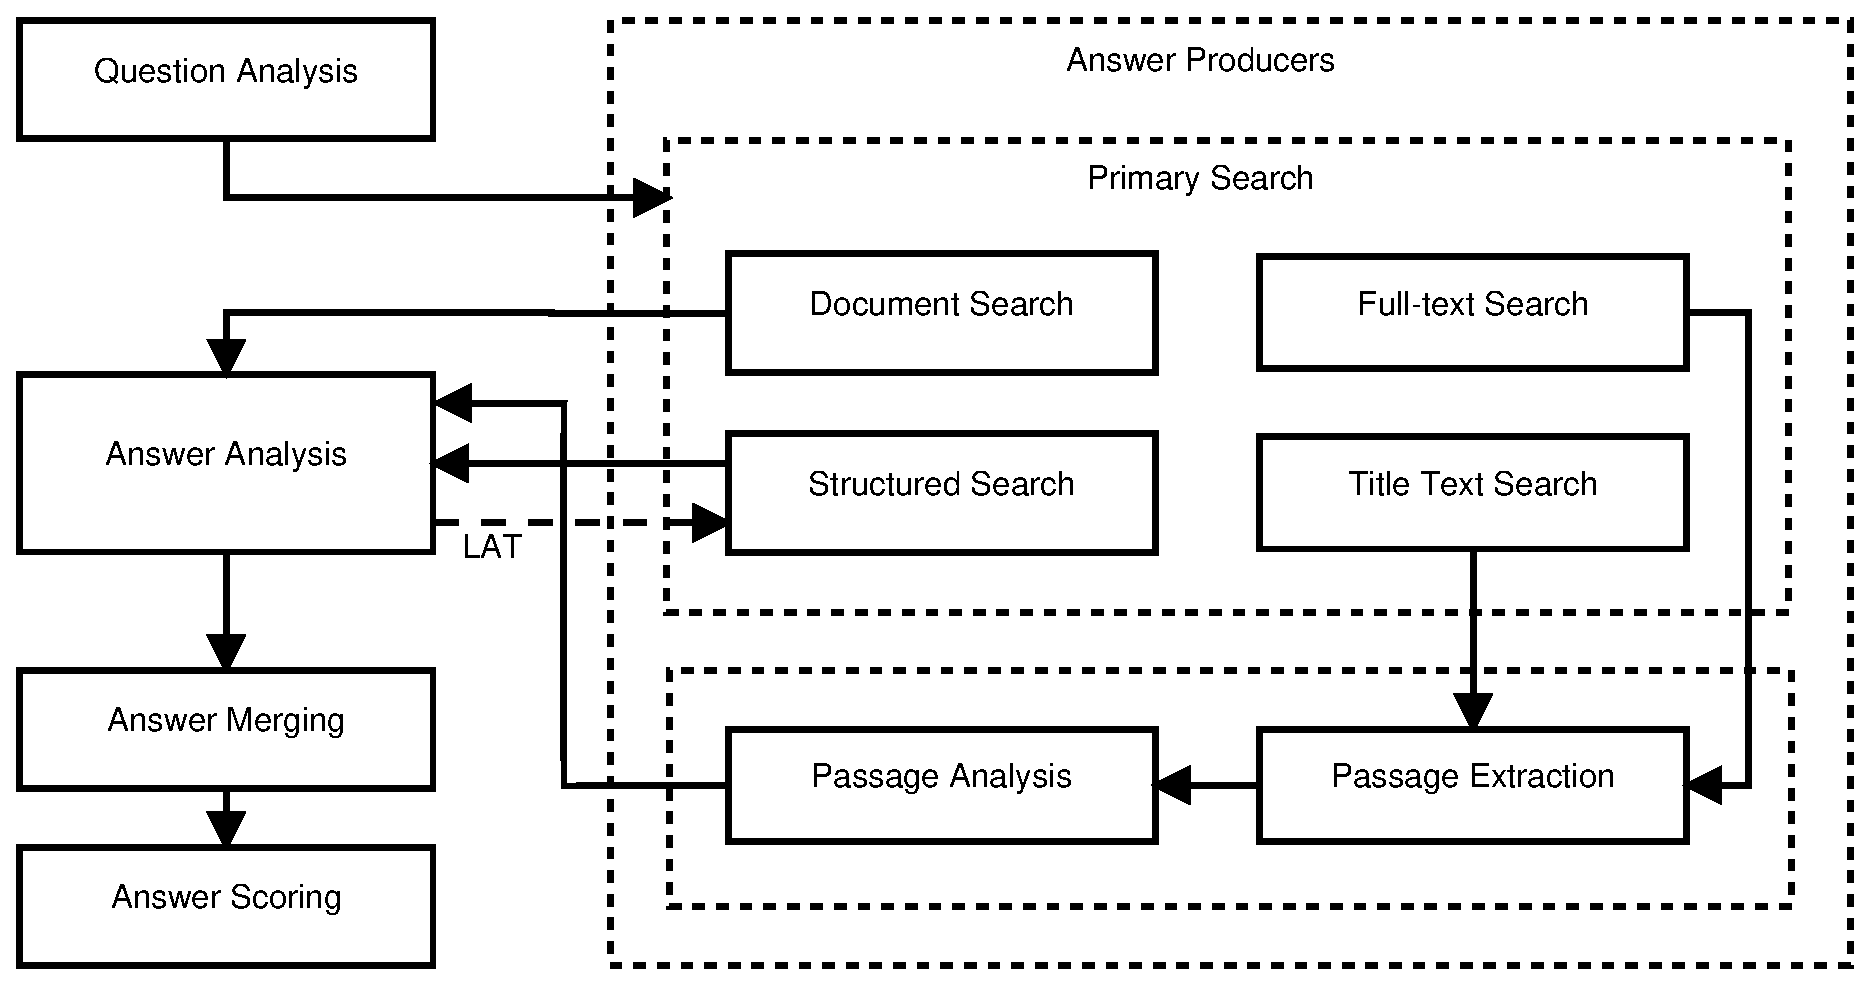
\includegraphics{yodaqa-arch.eps}}
%\vspace*{-0.75cm}
\caption{The general architecture of the YodaQA pipeline.  Present but unused final pipeline portions not shown.
TODO: Collapse answer production.  Plot sub-graphs with pipeline pieces in more detail.}
\label{fig:arch}
\end{center}
\end{figure}%\vspace{5mm}

The system maps an input question to ordered list of answer candidates in a pipeline fashion,
with the flow as in Fig.~\ref{fig:arch}, encompassing the following stages:

\begin{itemize}
\item \textbf{Question Analysis} extracts natural language features from
	the input and produces in-system representations of the question.
\item \textbf{Answer Production} generates a set of candidate answers based on the question,
	by performing a \textbf{Primary Search} in the knowledge bases according to the question clues
	and either directly using the results as candidate answers
	or selecting the relevant passages (the \textbf{Passage Extraction})
	and generate candidate answers from these (the \textbf{Passage Analysis}).
\item \textbf{Answer Analysis} generates answer features based on detailed analysis (most importantly, lexical type determination and coercion to question type).
\item \textbf{Answer Merging and Scoring} consolidates the set of answers, removing duplicates and using a machine learned classifier to score answers by their features.
\item \textbf{Successive Refining} (optional) prunes the set of questions in multiple phases, interjecting some extra tasks (evidence diffusion and gathering additional evidence).%
\footnote{We do not include Successive Refining in our evaluation or include further details as it is not beneficial in our current setup.}
\end{itemize}

The basic pipeline flow is much inspired by the Deep\-QA model
of IBM Watson \citep{WatsonPipeline}.  Throughout the flow, answer features
are gradually accumulated and some results of early flow stages (especially
the question analysis) are carried through the rest of the flow.


\section{YodaQA Reference Pipeline}
\label{sec:yodaqarefpip}

The reference pipeline currently considers an English-language task
as outlined in the Introduction --- answering open domain
factoid questions, producing a narrowly phrased answer.
We base the answers on information retrieval from both
unstructured (English Wikipedia --- \textit{enwiki})
and structured (DBpedia \citep{dbpedia}, Freebase \citep{freebase})
knowledge bases.

In our pipeline, we build on existing third-party NLP analysis tools,
in particular Stanford CoreNLP (Segmenter, POS-Tagger, Parser) \citep{StanfordCoreNLP} \citep{StanfordNNParser},
OpenNLP (Segmenter, NER) \citep{OpenNLP} and LanguageTool (Segmenter, Lemmatizer).%
\footnote{\url{http://www.languagetool.org/}}%
\footnote{Sometimes, different pipeline components default to different
NLP backends to perform the same task, e.g.\ segmentation,
based on empirically determined best fit.}
NLP analysis backends are freely interchangeable thanks
to the DKPro UIMA interface \citep{DKPro}.
For semantic analysis, we also rely heavily on the WordNet lexicon \citep{WordNet}.

Our key design rule is avoidance of hand-crafted rules and heuristics,
instead relying just on fully-learned universal mechanisms;
we use just about 10 hard-coded rules at this point, mostly
in question analysis.

For a practical illustration of the pipeline processing
two particular example questions,
see Appendix~\ref{app:analysis}.


\subsection{Question Analysis}

The question analysis involves
producing a part-of-speech tagging and dependency parse of the question text,
recognizing named entities and
performing entity linking%
\footnote{Right now, entities are linked just by an exact match of the main or alias label.}
to concepts (as represented by \textit{enwiki} articles).
The question representation we produce is similar in spirit
to DeepQA \cite{WatsonQuestion}: a bag-of-features including
a set of clues (keywords, keyphrases and linked concepts),
possible lexical answer types and the selection verb.

\textbf{Clues} represent keywords in the question that determine its content
and are used to query for candidate answers.
Clues based on different question components are assigned different weight
(used in search retrieval and passage extraction, determined empirically) ---
in ascending other, all noun phrases, noun tokens and the selection verb (SV);
the LAT (see below); named entities and matched concepts;
the question sentence subject (determined by dependency parse).

\textbf{Focus} is the center point of the question sentence
indicating the queried object.
Six simple hand-crafted heuristics extract the focus based on the dependency parse.
``name of ---'' constructions are traversed.

\textbf{LAT} (Lexical Answer Type) describes a type of the answer that would fit the question.
This type is not of a pre-defined category but may be an arbitrary English noun,
like in the DeepQA system. \citep{WatsonTyCor}
The LAT is derived from the focus, except question words are mapped to nouns
(``where'' to ``location'', etc.)
and adverbs (like ``hot'') are nominalized (to ``temperature'') using WordNet relations.

\textbf{SV} (Selection Verb) represents the coordinating verb of the
question that selects the answer with regard to other clues (like ``born'',
``received'', etc.)

\subsection{Unstructured Knowledge Bases}

The primary source of answers in our QA system is keyword search in free-text knowledge base
(the \textit{enwiki} in our default setting).
While the knowledge base has no formal structure,
we take advantage of the organization of the \textit{enwiki} corpus
where entity descriptions are stored in articles that bear the entity name as title
and the first sentence is typically an informative short description of the entity.
Our search strategies are analogous to basic DeepQA free-text information retrieval methods \citep{WatsonIR}.
We use the Apache Solr\footnote{\url{http://lucene.apache.org/solr/}} search engine (frontend to Apache Lucene).

\textbf{Title-in-clue search} \citep{WatsonIR} looks for the question clues in the article titles,
essentially aiming to find articles that describe the concepts touched in the question.
The first sentences of the top six articles (which we assume is its summary)
are then used in passage analysis (see below).

\textbf{Full-text search} \citep{WatsonIR} runs a full-text clue search in the article texts and titles,
considering the top six results.
The document texts are split to sentences which are treated as separate passages
and scored based on sum of weights of clues occuring in each passage\footnote{%
The \textit{about-clues} which occur in the document title have their weight divided by four (as determined empirically).}%
\footnote{We also carry an infrastructure for machine learning models scoring candidate passages,
		but they have not been improving performance so far.};
the top three passages from each document are picked for passage analysis.

\textbf{Document search} \citep{WatsonIR} runs a full-text clue search in the article texts;
top 20 article hits are then taken as potential responses,
represented as candidate answers by their titles.

\textbf{Concept search} retrieves articles that have been linked to entities mentioned in the question.
The first sentence as well as passages extracted like in the full-text search are used for passage analysis.

Given a picked passage, the \textbf{passage analysis} process executes an NLP pipeline and generates candidate answers;
currently, the answer extraction strategy entails simply converting all named entities and noun phrases to candidate answers.
Also, object constituents in sentences where subject is the question LAT are converted to candidate answers.

\subsection{Structured Knowledge Bases}

Aside of full-text search, we also employ structured knowledge bases organized in RDF triples;
in particular, we query the DBpedia \texttt{ontology} (curated) and \texttt{property} (raw infobox)
namespaces and the Freebase RDF dump.

For each concept
linked to an in-question entity, we query for predicates with this concept as a subject%
\footnote{All our knowledge bases are linked to \textit{enwiki}.}
and generate candidate answers for each object in such a triple, with the predicate label seeded as one LAT of the answer.

%For performance reasons, we limit the number of queried Freebase topics to 5 and retrieve only 40 properties per each;
%due to this limitation, we have manually compiled a blacklist of skipped
%``spammy'' properties based on past system behavior analysis
%(e.g.\ location's \textit{people\_born\_here} or music artist's \textit{track}).

Furthermore, we have trained a multi-label classifier (logistic regression)
that predicts \textit{property paths}
likely connecting an identified in-question concept with the answer in the knowledge base
graph based on particular forms in question representation. \cite{LeanFreebaseYao}
Unlike \cite{LeanFreebaseYao}, we consider long property paths as
Freebase is organized such that finding related concepts
often requires traversing intermediate nodes representing relationshibs (e.g.\ siblinghood).

\subsection{Answer Analysis}

In the answer analysis, the system takes a closer look at the answer snippet
and generates numerous features for each answer.
The dominant task here is type coercion,
i.e.\ checking whether the answer type matches the question LAT.

The answer LAT is produced by multiple strategies:
\begin{itemize}
	\item Answers generated by a named entity recognizer have LAT corresponding to the triggering model;
		we use stock OpenNLP NER models \textit{date}, \textit{location}, \textit{money}, \textit{organization}, \textit{percentage}, \textit{person} and \textit{time}.
	\item Answers containing a number have a generic \textit{quantity} LAT generated.
	\item Answer focuses (the parse tree roots) are looked up in WordNet and \textit{instance-of} pairs are used to generate LATs (e.g.\ \textit{Einstein} is \textit{instance-of} \textit{scientist}).
	\item Answer focuses are looked up in DBpedia and its ontology is used to generate LATs.
	\item Answers originating from a structured knowledge base carry the property name as an LAT.
\end{itemize}

Type coercion between question and answer LATs is performed using the WordNet
hypernymy relation --- i.e.\ \textit{scientist} may be generalized to \textit{person}, or \textit{length} to \textit{quantity}.
We term the type coercion score \textbf{WordNet specificity} and exponentially decrease it
with the number of hypernymy traversals required.
Answer LATs coming from named entity recognizer and quantity are not generalized.
We never generalize further once within the \texttt{noun.Tops} WordNet domain and
based on past behavior analysis, we have manually compiled a further blacklist
of WordNet synsets that are never accepted as coercing generalizations
(e.g. \textit{trait} or \textit{social group}).

The generated features describe the origin of the answer (data source, search result score, clues of which type matched in the passage, distance-based score of adjacent clue occurences, etc.), syntactic overlaps with question clues and type coercion scores (what kind of LATs have been generated, if any type coercion succeeded, what is the WordNet specificity and whether either LAT had to be generalized).

\subsection{Answer Merge-and-Score}

The merging and scoring process also basically follows a simplified DeepQA approach \citep{WatsonScoring}.
Candidate answers of the same text (up to basic normalization, like \textit{the-} removal) are merged;
element-wise maximum is taken as the resulting answer feature vector
(except for the \texttt{\#occurences} feature, where a sum is taken).
To reduce overfitting, too rare features are excluded
(when they occur in less than $1\%$ questions and $0.1\%$ answers).

Supplementary features are produced for each logical feature --- aside of the original value,
a binary feature denoting whether a feature has \textit{not} been generated
and a value normalized over the full set of answers
so that the distribution of the feature values over the answer
has mean 0 and standard deviation 1.
The extended feature vectors are converted to a score $s \in [0,1]$
using a logistic regression classifier.%
\footnote{An alternative gradient-boosted decision forest classifier is also
	available, but it is not beneficial in the default evaluation scenario yet.}
The weight vector is trained on the gold standard of a training dataset,
employing L2 regularization objective.  To strike a good precision-recall
balance, positive answers (which are about $p=0.03$ portion of the total)
are weighed by $0.5/p$.

\subsection{Successive Refining}

The pipeline contains support for additional refining and scoring phases.
By default, after initial answer scoring,
only the top 25 answers are kept with the intent of reducing noise for the next answer scoring classifier.
Answers are compared and those overlapping syntactically (prefix, suffix, or substring aligned with sub-phrase boundaries)
are subject to evidence diffusion where their scores are used as features of the overlapping answers.
Another answer scoring would be then performed, and the answer with the highest score is then finally output by the system.%
\footnote{There is also experimental support for additional evidence gathering phase, where the top 5 answers are looked up using the full-text search together with the question clues, and the number and score of hits are used as additional answer features and final answer rescoring is performed.  Nevertheless, we have not found this approach effective.}

However, while we have found these extra scoring steps beneficial with
weaker pipelines (in particular without the clue overlap features),
in the final pipeline configuration the re-scoring triggers significant
overfitting on the training set and we therefore ignore
the successive refining stage in the benchmarked pipeline.


\section{Performance Analysis}
\label{sec:results}

As we present performance analysis of our system,
we shall first detail our experimental setup;
this also includes discussion of our question dataset.

Then, we proceed with the actual results --- we measure the \textit{IR recall}
of the system (whether a correct answer has been generated and considered,
without regard to its score) and \textit{precision-at-one} (whether the
correct answer has been returned as the top answer by the system).
We find this preferrable to typical information retrieval measures like MRR or MAP
since in many applications, eventually only the single top answer output by the system
matters; however, we also show the \textit{mean reciprocial rank}
for each configuration and discuss the rank distribution of correct answers.

Aside of the performance of the default configuration, we also discuss
scaling of the system (extending the alotted answer time) and performance
impact of its various components (hold-out testing).

\subsection{Experimental Setup}

Our code is version tracked in a public GitHub repository
\url{https://github.com/brmson/yodaqa}, and the experiments presented
here are based on commit \texttt{TODO} (tagged as \texttt{v1.1}).
The quality of full-text search is co-determined by Solr version
(we use 4.6.0) and models of the various NLP components which are brought
in by DKPro version 1.7.0.
As for the knowledge bases, we use enwiki-20150112, DBpedia 2014,
Freebase RDF dump from Jan 11 2015, and WordNet 3.1.
Detailed instructions on setting up the same state locally (including
download of the particular dump versions and configuration files) are
distributed along the source code.

An automatic benchmark evaluation system is distributed as part of the
YodaQA software package.  The system evaluates the training and test questions
in parallel and re-trains the machine learning models before scoring the answers.
Therefore, in all the modified system versions considered below, a model trained
specifically for that version is used for scoring answers.

Our benchmark is influenced by two sources of noise.
First, the answer correctness is determined automatically by matching a predefined regex,
but this may yield both false positives and false negatives.%
\footnote{For example numerical quantities with varying formatting and units are notoriously tricky to match by a regular expression.}
Second, during training the models are randomly initialized and therefore their final
performance on a testing set flutters a little.

As a main benchmark of the system performance, we use a dataset of 430 training
and 430 testing open domain factoid questions.
(For system development, exclusively questions from the training set are used.)
This dataset is based on the public question answering benchmark from
the main tasks of the TREC 2001 and 2002 QA tracks
with regular expression answer patterns%
\footnote{\url{http://trec.nist.gov/data/qa/2001_qadata/main_task.html} and 2002 analogically.}
and extended by questions asked
to a YodaQA predecessor by internet users via an IRC interface.
This dataset was further manually reviewed by the author,
ambiguous or outdated questions were removed
and the regex patterns were updated based on current data.
We refer to the resulting 867 question dataset as \texttt{curated} and
randomly split it to the training and testing sets.\footnote{The remaining
7 questions are left unused for now.}

To further facilitate comparison of YodaQA to other systems,
we also benchmark its performance on the (i) original, unrevised and
unabridged TREC datasets
(even though the train/test splits might not be entirely compatible),
and (ii) the WebQuestions dataset \cite{WebQuestions}
(which represents several thousands of open domain factoid questions
tied to Freebase, popular as a semantic parsing benchmark).

\subsection{Benchmark Results}

TODO FIXME XXX

\begin{figure}[t]
% increase table row spacing, adjust to taste
\renewcommand{\arraystretch}{1.3}
\centering
\begin{tabular}{|c|cccc|}
\hline
Pipeline & IR Recall & Precision-at-1 & MRR & time \\ \hline \hline
default & 79.3\% & 32.6\% & 0.420 & 28.8s \\
% test  1119b6c 2015-03-09 Merge branch 'master... 144/289/430 33.5%/67.2% avgscore 0.504 mrr 0.424 avgtime 283643.667	+uv +uv
% test u1119b6c 2015-03-09 Merge branch 'master... 140/341/430 32.6%/79.3% avgscore 0.602 mrr 0.420 avgtime 283440.296
% test v1119b6c 2015-03-09 Merge branch 'master... 138/290/430 32.1%/67.4% avgscore 0.503 mrr 0.417 avgtime 283569.631
\hline
full-text scaling ($6\to12$ fetched results) & 82.3\% & 34.0\% & 0.430 & 50.0s \\
% test  e8e2f7b 2015-03-21 SolrFullPrimarySearc... 133/295/430 30.9%/68.6% avgscore 0.512 mrr 0.418 avgtime 12260.108	uv+ uv+
% test ue8e2f7b 2015-03-21 SolrFullPrimarySearc... 146/354/430 34.0%/82.3% avgscore 0.630 mrr 0.430 avgtime 11980.825
% test ve8e2f7b 2015-03-21 SolrFullPrimarySearc... 135/297/430 31.4%/69.1% avgscore 0.519 mrr 0.425 avgtime 12168.474

passage scaling ($3\to6$ picked passages) & 81.2\% & 31.4\% & 0.415 & 43.5s \\
% test  e1b3c91 2015-03-21 PassFilter: NUM_PICK... 137/296/430 31.9%/68.8% avgscore 0.509 mrr 0.419 avgtime 10368.150	v+u
% test ue1b3c91 2015-03-21 PassFilter: NUM_PICK... 135/349/430 31.4%/81.2% avgscore 0.616 mrr 0.415 avgtime 10088.654
% test ve1b3c91 2015-03-21 PassFilter: NUM_PICK... 146/294/430 34.0%/68.4% avgscore 0.516 mrr 0.432 avgtime 10275.724

document search scaling ($20\to40$) & 80.0\% & 31.6\% & 0.418 & 34.9s \\
% test  d8debbd 2015-03-21 SolrDocPrimarySearch... 135/292/430 31.4%/67.9% avgscore 0.499 mrr 0.410 avgtime 10859.761	u+v u+v
% test ud8debbd 2015-03-21 SolrDocPrimarySearch... 136/344/430 31.6%/80.0% avgscore 0.604 mrr 0.418 avgtime 10649.831
% test vd8debbd 2015-03-21 SolrDocPrimarySearch... 134/291/430 31.2%/67.7% avgscore 0.501 mrr 0.410 avgtime 10787.752

freebase scaling ($5\to10$ topics, $40\to80$ properties) & 79.8\% & 31.6\% & 0.416 & 29.8s \\
% test  6475b89 2015-03-22 FreebaseOntology: TO... 136/290/430 31.6%/67.4% avgscore 0.499 mrr 0.412 avgtime 6985.841
% test u6475b89 2015-03-22 FreebaseOntology: TO... 136/343/430 31.6%/79.8% avgscore 0.603 mrr 0.416 avgtime 6782.731
% test v6475b89 2015-03-22 FreebaseOntology: TO... 140/290/430 32.6%/67.4% avgscore 0.504 mrr 0.418 avgtime 6913.904

\hline
full-text hold-out & 49.5\% & 20.9\% & 0.277 & 5.8s \\
% test  cb27e81 2015-03-20 Merge branch 'master... 80/188/430 18.6%/43.7% avgscore 0.307 mrr 0.252 avgtime 1675.430	uv+
% test ucb27e81 2015-03-20 Merge branch 'master... 90/213/430 20.9%/49.5% avgscore 0.358 mrr 0.277 avgtime 1464.086
% test vcb27e81 2015-03-20 Merge branch 'master... 86/189/430 20.0%/44.0% avgscore 0.315 mrr 0.263 avgtime 1580.048

structured hold-out & 73.5\% & 29.1\% & 0.376 & 23.8s \\
% test  0659767 2015-03-20 YodaQA: Experimental... 113/265/430 26.3%/61.6% avgscore 0.448 mrr 0.362 avgtime 5443.057	uv+	vu+
% test u0659767 2015-03-20 YodaQA: Experimental... 125/316/430 29.1%/73.5% avgscore 0.546 mrr 0.376 avgtime 5261.876
% test v0659767 2015-03-20 YodaQA: Experimental... 125/267/430 29.1%/62.1% avgscore 0.461 mrr 0.380 avgtime 5371.852

type coercion hold-out & 79.3\% & 22.1\% & 0.314 & 30.0s \\
% test  a458fbf 2015-03-20 AnswerAnalysis: Expe... 90/246/430 20.9%/57.2% avgscore 0.388 mrr 0.304 avgtime 7249.693	uv+
% test ua458fbf 2015-03-20 AnswerAnalysis: Expe... 95/341/430 22.1%/79.3% avgscore 0.520 mrr 0.314 avgtime 7042.305
% test va458fbf 2015-03-20 AnswerAnalysis: Expe... 91/246/430 21.2%/57.2% avgscore 0.395 mrr 0.310 avgtime 7177.386

concept clues hold-out & 67.9\% & 23.0\% & 0.314 & 25.6s \\
% test  fdf189d 2015-03-20 QuestionAnalysis: Ex... 100/248/430 23.3%/57.7% avgscore 0.399 mrr 0.319 avgtime 6356.564	v+u
% test ufdf189d 2015-03-20 QuestionAnalysis: Ex... 99/292/430 23.0%/67.9% avgscore 0.490 mrr 0.314 avgtime 6104.581
% test vfdf189d 2015-03-20 QuestionAnalysis: Ex... 100/247/430 23.3%/57.4% avgscore 0.403 mrr 0.322 avgtime 6258.929

%external-resource LATs hold-out & 79.3\% & 22.1\% & 0.314 & 20.1s \\
% test  fe1b2e8 2015-03-20 AnswerAnalysis: Expe... 87/245/430 20.2%/57.0% avgscore 0.383 mrr 0.298 avgtime 5058.735	uv+
% test ufe1b2e8 2015-03-20 AnswerAnalysis: Expe... 95/341/430 22.1%/79.3% avgscore 0.520 mrr 0.314 avgtime 4888.693
% test vfe1b2e8 2015-03-20 AnswerAnalysis: Expe... 87/245/430 20.2%/57.0% avgscore 0.387 mrr 0.301 avgtime 4993.441

%fuzzy merging and evidence diffusion hold-out % & ...
% test  acbd992 2015-03-20 YodaQA pipeline: Exp... 129/290/430 30.0%/67.4% avgscore 0.497 mrr 0.405 avgtime 7364.049	uv+
% test uacbd992 2015-03-20 YodaQA pipeline: Exp... 139/341/430 32.3%/79.3% avgscore 0.602 mrr 0.420 avgtime 7131.604
% test vacbd992 2015-03-20 YodaQA pipeline: Exp... 135/290/430 31.4%/67.4% avgscore 0.503 mrr 0.413 avgtime 7276.565

clue overlap test hold-out & 79.3\% & 29.5\% & 0.390 & 30.1s \\
% test  65f5635 2015-03-20 AnswerAnalysis: Expe... 138/291/430 32.1%/67.7% avgscore 0.496 mrr 0.413 avgtime 7624.839	v+u
% test u65f5635 2015-03-20 AnswerAnalysis: Expe... 127/341/430 29.5%/79.3% avgscore 0.587 mrr 0.390 avgtime 7421.990
% test v65f5635 2015-03-20 AnswerAnalysis: Expe... 138/293/430 32.1%/68.1% avgscore 0.502 mrr 0.416 avgtime 7552.017
\hline
\end{tabular}
\vspace*{-0.2cm}
\caption{Benchmark results of various pipeline variants on the \textit{curated} test dataset.
MRR is the Mean Reciprocal Rank $|Q|\cdot\sum_{q\in Q}{1/r_q}$, time is the average time spent answering one question.}
\label{fig:bench}
\end{figure}

\begin{figure}[t]
\begin{center}
\resizebox{85mm}{!}{\includegraphics{ranks.eps}}
\vspace*{-0.75cm}
\caption{Number of questions $x$ that output the correct answer ranked at least $y$.}
\label{fig:ranks}
\end{center}
\end{figure}%\vspace{5mm}

Benchmark results over various pipeline configurations are laid out in Fig.~2. %\ref{fig:bench}.
Aside of the general performance of the system,
it is instructive to look at the histogram of answer ranks
for the default pipeline, shown in Fig.~\ref{fig:ranks}.
We can observe that while precision-at-one is 32.6\%,
precision-at-five is already at 52.7\% of test questions.

The information retrieval parameters of the default pipeline are selected so
that answering a question takes about 30s on average on a single core of
AMD FX-8350 with 24GB RAM and SSD backed databases.
(Note that no computation pre-processing was done on the knowledge bases or datasets;
bulk of the time per question is therefore spent querying the search engine and parsing sentences,
making it an accurate representation of time spent on previously unseen questions.)
By raising the limiting
parameters, we can observe further IR recall increase, and in case of considering
more full-text search results, also a solid precision improvement.  Our system
could therefore meaningfully make use of further computing resources.

We also benchmarked performance with various components of the pipeline
disabled.  We can see that the full-text and structured knowledge bases
are complementary to a degree, but the full-text base is eventually
a much stronger answer source for our system.  Type coercion and detection
of the concept clues in the question are both important heuristics for
our QA system.

Comparison of performance across multiple systems is currently non-trivial,
unfortunately, as there is no universally agreed experimental setup so far
and not even published results on the TREC datasets
from the years we use are readily available.
OpenEphyra seemed to typically achieve precision-at-one of ``above 25\%'' on
the TREC datasets including our years according to \citep{Ephyra2006}.
In the Answer Sentence Selection task \citep{WangQAGrammar},
Jacana and similar textual entaliement systems are reported%
\footnote{See the \textbf{ACL Wiki} topic \textit{Question Answering (State of the art)}.}
to achieve MRR around 0.750 but this task represents
a significant restriction upon the general end-to-end QA pipeline.

\section{System Performance}

In Fig.~\ref{fig:bench}, we compare various performance measures
with the most relevant previously published systems
(on the TREC dataset, as reported in the respective papers),
with ours benchmarked on non-curated version of the TREC 2002, 2003 dataset test split.

\begin{figure}[t]
%% increase table row spacing, adjust to taste
%\renewcommand{\arraystretch}{1.3}
\centering
\begin{tabular}{|c|cccc|}
\hline
System & Precision-at-1 & IR Recall & F1 & MRR \\ \hline
LLCpass03 \citep{LCC} (hand-crafted system) & 68.5\% & & & \\
AskMSR \citep{AskMSR} (web-search system) & 61.4\% & & & 0.507 \\ \hline
OpenEphyra \citep{Ephyra2006} (hand-crafted OSS) & ``above 25\%'' & & & \\
JacanaIR \citep{TreeEditIR2013Yao} (modern fully-learned OSS) & & & & 0.299$^*$ \\
OQA \citep{OQA} (modern fully-learned OSS) & & & 29\%$^{**}$ & \\ \hline
\textbf{YodaQA v1.0} & 25.1\% & 62.2\% & 35.8\% & 0.323 \\
\hline
\end{tabular}
\vspace*{-0.2cm}
\caption{Benchmark results of some relevant systems on the unmodified TREC dataset.\quad
$^*$ answer-bearing sentence retrieval\quad
$^{**}$ sub-sampled dataset with manual evaluation}
\label{fig:bench}
\end{figure}

\chapter{Future Work}
\label{ch:plan}

TODO

\chapter{Conclusion}
\label{ch:concl}

In this report, I have proposed a doctoral thesis on the topic
of factoid question answering.
So far, I have built a question answering system that exhibits
TODO performance and is still rapidly improving.  I have also
managed to reproduce state-of-art results in some of the sub-tasks
and identified and proposed a few tasks on my own that are tied
to building a state-of-art system in a real-world setting.

In my thesis, apart of describing my system building work, I would
like to focus particularly on research connected to the Information Extraction
portion of the system.

As discussed above, vector embeddings are a booming area of semantic
NLP research with their ability to numerically capture meaning nuances,
and based on the presented survey of the field, I believe looking into
vector embedding approaches when manipulating natural text
(analyzing the question, understanding answer-bearing
passages and relation labels) is a highly promising area of research.
Some scientific problems that I would like to tackle are connected
to the current limitations of vector embeddings themselves.
This includes building compound vector embeddings conveying
the meaning of a whole sentence rather than individual words,
and
exploring ways to embed or tie named entities, numerical quantities
and other arbitrary data to the conventional embeddings.

Other scientific problems related to Information Extraction that
I plan to explore are in particular testing various relation
extraction strategies in the unstructured knowledge base context
and improving performance in this sub-task.
My sight is also set at tasks beyond basic factoid QA like performing basic inference,
though it is unclear if it will eventually fall in the scope of my
thesis as well.

However, improving the system performance might lead to interesting
results in other parts of the system, involving Entity Linking,
Information Retrieval, Result Ranking etc.

In summary, I would like to propose a thesis studying
\textbf{Semantic Methods in Question Answering}.

\section{Acknowledgements}

I would like to thank my main supervisor Dr. Petr Pošík
for his guidance, support, but also giving me the freedom to
eventually take a different direction of scientific pursuit
than we originally planned.
I would also like to thank my specialist supervisor Dr. Jan Šedivý
for supporting me in this new topic of research, his result-focused
guidance and giving me great opportunities to boost the development
of my system.


\appendix
\chapter{Portfolio-Based Optimization}
\label{app:opt}

The initial focus of my doctoral research
was developing algorithm portfolio strategies
with applications particularly in continuous black-box optimization.
The results of my work have been a software framework for experiments
\citep{cocopf}
and two results published at top-tier conferences \citep{Baudis2014PPSNOnlinePortfolios,Baudis2015GECCO}.
This research had been primarily supervised by Dr. Petr Pošík.

Let us consider the problem of finding a minimum value of a continuous
real-parameter function that has inaccessible analytical form.%
\footnote{No analytical form implies that we do not have information
e.g.\ on the derivatives of the function, except approximating
them numerically.}
This is a rich area of research that produced many algorithms over
the last 50 years --- from the venerable Nelder-Mead simplex
algorithm \citep{NM1} to various gradient descent methods to
population-based methods.

\section{Online Black-box Algorithm Portfolios}

The key question in the face of such variety of optimization
algorithms is ``which algorithm should I choose?''
Unified comparison benchmarks \citep{COCO1}
can help determining the best option for a particular function class.
However, if a function is truly ``black-box'' and its features
are hard to predict, an automated process with minimum overhead
is certainly desirable.

The problem of algorithm selection is not new \citep{Rice}
and was so far popular mainly when applied to
combinatorial problem solvers \citep{combpfsurvey}.
In my work, I adopted the prism of algorithm portfolios \citep{algportfolios}
with \textit{online} selection.%
\footnote{The concept of offline selection also occurs in the literature,
	when we assume a stream of function instances and apply just a single
	algorithm on each of the instances.}
That is, multiple diverse optimization algorithms are applied
to the given function instance simultaneously, with the best
performers quickly gaining the largest time allocation (that is,
the chance to perform the most optimization steps).

Deciding which algorithm to apply in each step of the portfolio
optimization is essentialy an instance of the well-known Multi-Armed
Bandit Problem, where a policy decides which algorithm to try next
based on their empirically determined expected reward.
I have built a modular Python framework \textbf{COCOpf} \citep{cocopf}
suitable both for research and application of this problem.

This helped me to identify fine structure of the problem
(particularly, I proposed a classification of functions based on
their in-portfolio behavior).
Further, I have built a reference portfolio of seven well-known
diverse optimization algorithms and based on performance evaluation
using the popular COCO optimization benchmark \citep{COCO1}, I have
identified a policy that significantly improves the baseline and
on well-behaved functions on average overperforms even the overally
best individual algorithm. This result was presented at the
PPSN 2014 conference. \citep{Baudis2014PPSNOnlinePortfolios}

\section{Minimizing Separable Functions by a Mix of Methods}

Another tier of research on how to best combine different optimization
algorithms concerns speeding up optimization of continuous black-box
\textit{separable} functions in particular.  I have closely cooperated
on this research with my supervisor, Dr. Petr Pošík.

Separable multivariate functions can be decomposed to a sum of univariate
functions, each parametrized solely by a single dimension of the input
vector.
For some very hard separable functions, exploiting separability
is the only way to quickly find the minimum and a natural idea to optimize
such functions is to use univariate optimization algorithms on individual
dimensions.
In \citep{PosikGECCO2009LineSearch}, Brent's method \citep{Brent1973} and the STEP algorithm \citep{STEP} were used to separately optimize the function along each dimension.
Brent's method was shown to be fast in case of unimodal functions, but due to its local nature it fails on multimodal functions.
The global STEP method was able to solve both the uni- and multimodal functions, but needed much larger number of function evaluations.
Moreover, their multidimensional variants were constructed inefficiently: the dimensions were optimized sequentially, one by one.

We have built on the above mentioned methods, and contributed two improvements:

\begin{enumerate}
	\item We combined Brent's method and STEP into a single algorithm which converges faster than STEP (in many cases, it is almost as fast as Brent's method), while it preserves the global search ability of STEP (thus solving a larger proportion of functions than Brent's method, and often doing it faster).

	\item We suggested a better way of making a multidimensional variant of this method. As opposed to solving the 1D problem in all dimensions sequentially, we proposed to interleave the steps in individual dimensions, updating the full coordinates of sampled points based on results obtained in other dimensions so far.%
\footnote{Later, we found out about a similar recent work by Ilya Loschilov \cite{HCMA}, but our algorithm reaches better results.}
\end{enumerate}

Thus, we have introduced a new hybrid algorithm ``Brent-STEP'' combining
these two methods non-trivially and demonstrated that
on univariate and separable functions the hybrid algorithm
in general outperforms both of them,
in the univariate case often by a wide margin,
and that it is behaving robustly even when one of the constituent methods
is failing to converge.
This result was presented at the GECCO 2015 conference.
\citep{Baudis2015GECCO}

%\chapter{Examples: YodaQA Pipeline Analysis}
\label{app:analysis}

TODO: Revise and update.


\begin{figure}[t!]
% increase table row spacing, adjust to taste
\renewcommand{\arraystretch}{1.3}
\centering
\footnotesize
\begin{tabular}{|p{1.8cm}p{6cm}|}
\hline
Question Text & Who wrote Ender's Game? \\
Q. Analysis & \textbf{Focus:} who; \textbf{SV:} wrote; \textbf{LAT:} person \\
Question Clues & Ender's Game \textbf{(concept clue)}, wrote \\ \hline

Primary Search (DBpOnt.) & \textbf{author:} Orson Scott Card, \textbf{publisher:} Tor Books, \dots \\
Primary Search (DBpProp.) & (ibid), \textbf{cover artist:} John Harris, \textbf{Caption:} 2005, \dots \\
Primary Search (Freebase) & \textbf{Author} Orson Scott Card, \textbf{Characters} Valentine Wiggin, Hive Queen, \dots \\
Primary Search (concepts) & \textit{enwiki} Ender's Game \\
Primary Search (fulltext) %
	& \textbf{Query:} \texttt{+("wrote" OR titleText: "wrote")\^{}1.0 +("ender's Game" OR titleText:"ender's Game")\^{}1.1  ("wrote ender's Game "\textasciitilde4)\^{}2.1} \dots \\
	& \textbf{Found:} Ender's Game (series), Ender's Game, Ender's Game (film), Ender's Game (comics), Jane (Ender's Game), List of Ender's Game series planets \\
	& \textbf{Sample picked passages:} {\footnotesize Elaborating on characters and plot lines depicted in the novel, Card later wrote additional books to form the Ender's Game series.} \\
	& \dots {\footnotesize Valentine wrote an essay here comparing the priestly class to the skeletons of small vertebrates some time before Speaker for The Dead.} \\
Primary Search (titles) & Ender's Game, List of Ender's Game characters, Jane (Ender's Game), Ender's Game (short story), Ender's Game (film), Ender's Game (series) \\
	& \textbf{Sample first passage:} {\footnotesize "Ender's Game" is a 1985 military science fiction novel by American author Orson Scott Card.} \\
Primary Search (document) & Ender's Game (series), Elisabeth Hirsch, Orson Scott Card, Ender in Exile, Worthing Inn, Jane (Ender's Game), \dots \\ \hline

\textbf{Orscon Scott Card} & Structured primary search LAT \textit{author} (Wordnet hypernyms \textit{communicator}, \textit{person}, \textit{maker}, \textit{creator}); DBpedia LAT \textit{writer} (Wordnet hypernyms \textit{communicator}, \textit{person}); NER LAT \textit{person} \\
	& Successful type coercion match\textbf{!}, ``sharp'' (exact specific) match from NER LAT\textbf{!} \\
	& \textbf{occurences:} 19\textbf{!}, \textbf{origins:} document title, concept\textbf{!}, first passage, noun phrase, named entity, multiple origins, \textbf{other:} adjecent to a concept clue mention, no clue text overlap\textbf{!} \\
\textbf{Jane} & Structured primary search LAT \textit{character} (Wordnet hypernyms \textit{imaginary being}, \textit{creativity}, \textit{person}, \textit{message} and 36 others); NER LAT \textit{person} \\
	& Successful type coercion match\textbf{!}, ``sharp'' (exact specific) match from NER LAT\textbf{!} \\
	& \textbf{occurences:} 4, \textbf{origins} document title, first passage, noun phrase, named entity, multiple origins,
	\textbf{other:} no clue text overlap\textbf{!} \\ \hline

Final Answers & \textbf{Orson Scott Card} (0.99), Neal Shusterman (0.96), Elisabeth Hirsch (0.96), American author Orson Scott Card (0.96), \dots, List of Ender's Game series planets (0.94), Gavin Hood (0.94), Print (0.93), Jane (0.91), \dots \\ \hline
\end{tabular}
\vspace*{-0.2cm}
\caption{A sample of the pipeline process when (correctly) answering a training question. \textbf{!} indicates particularly distinguishing features.}
\label{fig:exEnder}
\end{figure}

\begin{figure}[t!]
% increase table row spacing, adjust to taste
\renewcommand{\arraystretch}{1.3}
\centering
\footnotesize
\begin{tabular}{|p{1.8cm}p{6cm}|}
\hline
Question Text & What is the name of the famous dogsledding race held each year in Alaska? \\
Q. Analysis & \textbf{Focus:} name; \textbf{SV:} held; \textbf{LAT:} race
	(by Wordnet hypernym: \textit{contest}, \textit{event}, \textit{biological group}, \textit{canal} and 9 others) \\
Question Clues & name, Alaska \textbf{(concept clues)}, race, held, famous, dogsledding, race, year \\ \hline

Primary Search (DBpOnt.) & \textbf{area Total:} 1717854.0, \textbf{country:} United States, \dots \\
Primary Search (DBpProp.) & (ibid), \textbf{West:} Chukotka, \textbf{Income Rank:} 4, \dots \\
Primary Search (Freebase) & \textbf{Date Founded} 1959-01-03, \textbf{Capital} Juneau, \dots \\
Primary Search (concepts) & \textit{enwiki} Alaska, Name \\
	& \textbf{Sample picked passages:} Various races are held around the state, but the best known is the Iditarod Trail Sled Dog Race, a 1150 mi trail from Anchorage to Nome (although the distance varies from year to year, the official distance is set at 1049 mi). \\
	& \dots Automobiles typically have a binomial name, a "make" (manufacturer) and a "model", in addition to a model year, such as a 2007 Chevrolet Corvette.\\
Primary Search (fulltext) & \textbf{Query:} \texttt{("the name of the famous dogsledding race held each year in Alaska" OR titleText:\dots)\^{}2.7 +("name" OR titleText:"name")\^{}2.6} \dots \\
	& \textbf{Found:} List of New Hampshire historical markers \\
Primary Search (titles) & Name of the Year, Danish Sports Name of the Year, List of organisms named after famous people, Alaska!, Alaska, Race of a Thousand Years \\
	& \textbf{Sample first passage:} The 2000 Race of a Thousand Years was an endurance race and the final round of the 2000 American Le Mans Series season. \\
Primary Search (document) & List of New Hampshire historical markers \\ \hline

\textbf{The 2000 Race of a Thousand Years} %
	& \textbf{Focus:} Race; DBpedia LAT \textit{automobile race}, \textit{auto race in australia}, \textit{new year celebration}, \textit{quantity} LAT \\
	& Successful type coercion match\textbf{!}, ``sharp'' (exact specific) match\textbf{!} \\
	& \textbf{occurences:} 1, \textbf{origins:}  first passage, noun phrase, \textbf{other:} adjecent to an LAT clue mention\textbf{!}, containing clue text \\
\textbf{Iditarod Trail Sled Dog Race} %
	& \textbf{Focus:} Race; DBpedia LAT \textit{sport}, \textit{sport in alaska}, \textit{alaska}, \textit{winter sport}, \textit{attraction}; (N.B. no \textit{race} LAT) \\
	& Successful type coercion match, loose match by generalization of \textit{attraction} to \textit{social event}\textbf{!} \\
	& \textbf{occurences:} 1, \textbf{origins}   passage by various clues, noun phrase,
	\textbf{other:} suffixed by clue text \\ \hline

Final Answers & The 2000 Race of a Thousand Years (0.97), --01-03 (0.94), List of New Hampshire historical markers (0.93), a binomial name, a "make" (manufacturer) and a "model", in addition to a model year, such as a 2007 Chevrolet Corvette (0.90), \textbf{the Iditarod Trail Sled Dog Race} (0.89), Various races (0.83), \dots \\ \hline
\end{tabular}
\vspace*{-0.2cm}
\caption{A sample of the pipeline process when (not quite correctly) answering a training question. \textbf{!} indicates particularly distinguishing features.}
\label{fig:exIditarod}
\end{figure}


\bibliographystyle{plainnat}
\bibliography{qa,opt}

\end{document}
